\chapter{Wavelength calibration}
\label{sec:wavelength}

This chapter uses the orders, slits, arcs and reduction names defined in the Conventions, p.~\pageref{sec:conventions}. It shows
that the archive wavelength scale has two separate problems: the arc solution has no lines near H$\beta$ and
H$\alpha$, and the wavelength zero point of a compact object in the 6\,arcsec slit changes with its position in the
slit. We correct both.

\section{How \banzai{} calibrates wavelengths}
\label{sec:wl_banzai}
\banzai{} derives the wavelength solution from the arc of each block in five steps. (1) It collapses each order along
the slit, following an assumed line tilt, and finds and identifies the emission peaks. (2) It measures the centroid of each
bright, isolated line in every row with a Gauss--Hermite profile \citep{Cappellari2017}, and fits blended lines with a
fixed line-spread function. (3) For each line it fits a straight line $x=a+b\,y_{\rm o}$, where $x$ is the column,
$y_{\rm o}$ the row relative to the order centre, and the slope $b$ gives the tilt of the line. (4) It fits the column
$x(\lambda)$ of the lines as a Legendre series in wavelength, of degree 5 in the red order and 2 in the blue in
\banzai{}~1.1.0 (the 1.0.1 archive products use degrees 4 and 2). (5) It inverts this to obtain $\lambda(x)$. At COJ
the tilt is a constant ($\approx8.2^\circ$). The final fit has no outlier rejection. There is also no per-exposure
correction of the zero point for flexure or for the position of the object in the slit: every science frame inherits
the solution of its arc.

\section{The arc line list leaves the H$\beta$ and H$\alpha$ regions unconstrained}
\label{sec:wl_lines}
Of the 68 lines in the \banzai{} arc-line catalogue, 33 are used in the fit. In the blue order the solution rests on
Hg lines only: 3650/3663 (a blend), 4047, 4078 and 4358\,\AA, and then 5461, 5770 and 5791\,\AA{}. There is no line
between 4358 and 5461\,\AA{}, exactly where H$\beta$ and [O\,{\sc iii}] fall for $z\lesssim0.1$. The red order
starts at $\approx4550$\,\AA{}, but its first used line is at 5461\,\AA{}, so the solution at 4550--5461\,\AA{} is
an extrapolation. The red order also has no line between 5791 and 6965\,\AA{}, where H$\alpha$ falls for
$z\approx0.05$. The Zn lines that would fill the blue gap are disabled in the \banzai{} line list, with the comment
``removed until we start turning on the Zn lamp again''.

To see which other lines are present, we collapsed all 64 raw arcs (Table~\ref{tab:data}) along the slit using the
2-d wavelength map of a science frame, and aligned them by cross-correlation. The night-to-night shifts are
1.07\,\AA{} rms in the red order and 0.49\,\AA{} in the blue. Three facts follow (Fig.~\ref{fig:arcs}):
\begin{enumerate}
\item[(i)] Hg\,4916 is detected in every single 60\,s arc in both orders, and Ar\,6416, 6677 and 6753/6767 in the red
order, so no stacking is needed to use them.
\item[(ii)] Although the Zn lamp is ``on'' in 63 of the 64 headers, no Zn line is detected, even in the stack of all
64 arcs.
\item[(iii)] Through the 6\,arcsec slit every line is a top-hat (the image of the slit) $\approx51$\,\AA{} wide in the
red order and $\approx25$\,\AA{} in the blue, so many neighbouring lines blend.
\end{enumerate}

\begin{figure}[!htbp]
\centering
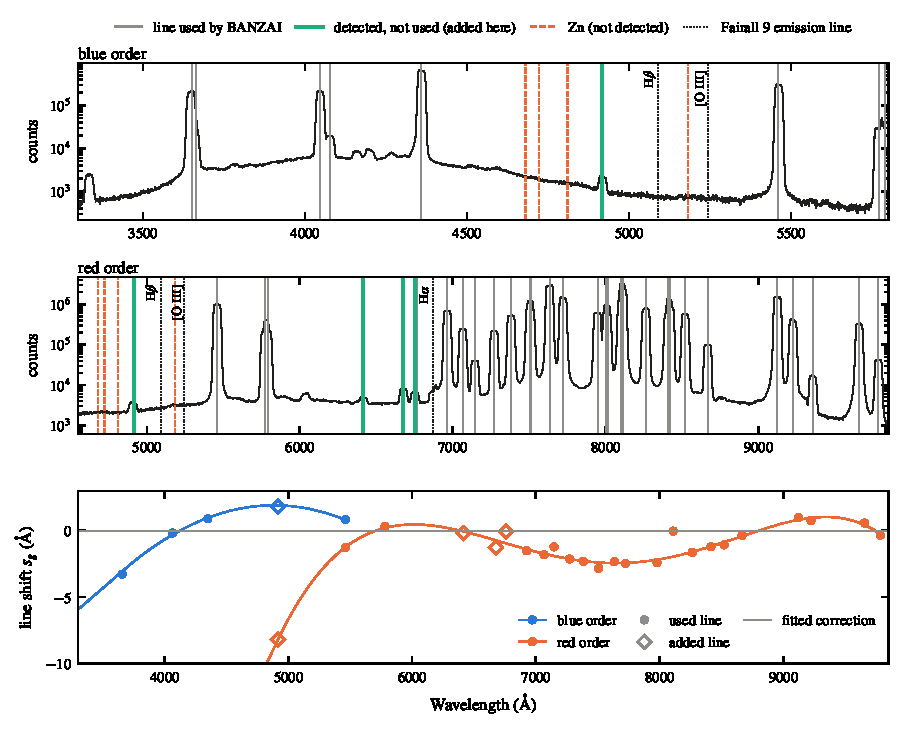
\includegraphics[width=\textwidth]{figures/fig_arcs.pdf}
\caption{Arc lines. Top and middle: one 60\,s arc (6\,arcsec slit) in the blue and red orders. Grey: lines used by
\banzai; aqua: lines detected but not used (Hg\,4916, Ar\,6416, 6677, 6753); dashed orange: Zn lines (lamp ``on''
in the headers, not detected); dotted: H$\beta$, [O\,{\sc iii}] and H$\alpha$ of Fairall~9. Bottom: shift $s_g$ of each
line group (eq.~\ref{eq:arcgroup}) on the \banzai{} solution of 2026-10-08 (circles: used lines; open diamonds: added
lines) and the fitted correction (eq.~\ref{eq:arccorr}). The red order's extrapolated end is off by $-8$\,\AA{} at
Hg\,4916.}
\label{fig:arcs}
\end{figure}


\section{Arc refit with the unused lines}
\label{sec:wl_refit}
For the archive products (improved v1) we measured the error of the archive solution at all detected lines and
corrected it afterwards. Each raw arc is overscan-subtracted and trimmed. It is then collapsed with the frame's own
2-d wavelength map, which already contains the line tilt: all pixels within 30 rows of the order centre are averaged
in wavelength bins of half a pixel. Lines that blend are measured together, in \emph{groups} $g$ with laboratory
wavelengths $\lambda_{g,j}$ (Table~\ref{tab:groups}), with the model
\begin{equation}
M_g(\lambda) = c_0 + c_1\frac{\lambda-\bar\lambda_g}{100} + \sum_j A_j\,B(\lambda;\lambda_{g,j}+s_g,W,\sigma),
\label{eq:arcgroup}
\end{equation}
\begin{equation}
B(\lambda;\mu,W,\sigma)=\frac{1}{2}\left[\mathrm{erf}\!\left(\frac{\lambda-\mu+W/2}{\sqrt2\,\sigma}\right)
 -\mathrm{erf}\!\left(\frac{\lambda-\mu-W/2}{\sqrt2\,\sigma}\right)\right].
\label{eq:boxcar}
\end{equation}
Here $c_0+c_1(\lambda-\bar\lambda_g)/100$ is a linear background, with $\bar\lambda_g$ the mean wavelength of the
group, and $B$ is a top-hat of the width $W$ of the slit image convolved with a Gaussian of width $\sigma$. There is
one such profile per line, at the laboratory separations, with free amplitudes $A_j\ge0$ and a common shift $s_g$:
the measured minus the laboratory wavelength on the solution being tested. The initial width is
$W=8.5$\,\AA\,arcsec$^{-1}$ (red) or 4.25\,\AA\,arcsec$^{-1}$ (blue) times the slit width. Two lines closer than
$0.3W$ cannot be separated, because their amplitude ratio is degenerate with $s_g$. If both catalogue strengths are
known, they are merged into one line at their strength-weighted mean wavelength; if a strength is unknown, both are
kept with free amplitudes. A group is accepted if the fit converged, $|s_g|<14.5$\,\AA{} and its peak exceeds 10
times the residual noise.

The correction is a weighted Legendre series fitted to the group shifts,
\begin{equation}
\Delta\lambda(\lambda)=\sum_{k=0}^{K}d_k\,L_k(\tilde\lambda),\qquad
w_g = \left(\sigma_{s_g}^2+0.3^2+\delta_g^2\right)^{-1},
\label{eq:arccorr}
\end{equation}
where $L_k$ are the Legendre polynomials with coefficients $d_k$, $K=5$ (red) and 2 (blue), $\tilde\lambda$ is the
wavelength mapped to $[-1,1]$, and $w_g$ is the weight of group $g$. In the weight, $\sigma_{s_g}$ is the statistical
error of $s_g$ from the fit, 0.3\,\AA{} is an error floor and $\delta_g$ is an extra systematic error for
unresolved blends (0.5--1\,\AA{}, Table~\ref{tab:groups}). Groups deviating by more than $4\sigma$ are rejected
iteratively. Outside the wavelength range of the accepted groups the correction is continued linearly from its end
values and slopes, so that a degree-5 fit never extrapolates wildly. The corrected wavelength is
$\lambda'=\lambda-\Delta\lambda(\lambda)$.

The fit to one night's arc leaves residuals of 0.48\,\AA{} rms in the red order (median over nights; 23 groups) and
0.10\,\AA{} in the blue (4 groups). The archive red-order solution is wrong by $\approx-8$\,\AA{} at Hg\,4916 and
$\approx-3$\,\AA{} at 5240\,\AA{} (Fig.~\ref{fig:arcs}, bottom). The shape of the arc solution is stable: after
removing each night's zero point, the solutions of the 50 frames agree to $<0.4$\,\AA{} over most of each order. We
therefore apply the \emph{median} of the nightly corrections to every frame; using each night's own fit only adds fit
noise (Section~\ref{sec:results_wl}).

This refit was designed for the archive products (improved v1). The arc fit of \banzai{}~1.1.0, run from the raw
frames, is already far better than the 1.0.1 solution: on the same arcs it is off at the unused lines by at most
0.6\,\AA{} instead of $-8$\,\AA. In the final pipeline (improved v3) the unused lines are added to the arc fit itself.
This brings the remaining error at Hg\,4916 to $\approx0.1$\,\AA{} in the red order (Section~\ref{sec:sites_arcs}),
and no refit afterwards is needed.

\section{The zero point of the object's light}
\label{sec:wl_zp}
The arc and the night sky fill the slit; a compact object does not. In a wide slit the wavelength zero point of the
object therefore depends on where it sits across the slit. A displacement $\Delta\theta$ across the slit moves its
spectrum by $\Delta x=\Delta\theta/0.337''$ pixels, i.e. by $\approx10$\,\AA{} per arcsec in the red order. Neither
the arc nor the sky lines can measure this, because both fill the slit. The telluric absorption bands can
(Section~\ref{sec:diag_tell}): they are imprinted on the object's own light, at wavelengths fixed by the atmosphere.
For each band $b$ we measure the shift $s_b$ of the band in the object spectrum relative to a transmission template
(eq.~\ref{eq:tell}). We subtract the band's offset $o_b$ relative to the O$_2$ A band (Table~\ref{tab:bands},
calibrated on the 18 EG\,21 spectra after the arc refit). We then combine the bands into one red-order shift,
\begin{equation}
s_{\rm red}=\frac{\sum_b \omega_b\,(s_b-o_b)/(\sigma_{s_b}^2+0.5^2)}{\sum_b \omega_b/(\sigma_{s_b}^2+0.5^2)},
\label{eq:tellcomb}
\end{equation}
where $\sigma_{s_b}$ is the error of $s_b$, 0.5\,\AA{} is an error floor, and $\omega_b$ is a weight per band (1 for
the A band, 0.5 for the B band and the H$_2$O band at 7200\,\AA, 0.25 for the H$_2$O band at 9300\,\AA). Bands
deviating by more than $3\sigma$ are rejected iteratively. Both orders image the same slit, so the blue-order shift in pixels is the red-order one times the ratio $\rho$ of
the anamorphic magnifications of the two orders:
\begin{equation}
s_{\rm blue} = \rho\,\frac{s_{\rm red}}{D_{\rm red}}\,D_{\rm blue},\qquad \rho=1.13,
\label{eq:transfer}
\end{equation}
with $D$ the dispersion of each order (\AA\,pixel$^{-1}$). We measured $\rho$ once, as the slope of the blue-order
[O\,{\sc iii}] pixel shift against the red-order A-band pixel shift in the Fairall~9 frames (slope 1.13--1.14,
$r=0.99$, residual 0.2\,pixel); it is an instrument constant. The corrected wavelengths are
$\lambda''=\lambda'-s_{\rm order}$, with $s_{\rm order}$ equal to $s_{\rm red}$ or $s_{\rm blue}$. If no band is usable,
the zero point from the sky lines (Section~\ref{sec:diag_sky}) is used instead; this corrects flexure but not the
position in the slit.

This method ties the wavelength scale to the telluric template, so its absolute zero point is that of the template.
It is uncertain by $\approx\pm4$\,\AA. On the standards the A band lies $-3.5\pm0.7$\,\AA{} from the sky lines (if
the standards are centred in the slit), whereas the [O\,{\sc iii}] lines of Fairall~9 imply $+3.9$\,\AA{} (if
[O\,{\sc iii}] is at the systemic redshift). This uncertainty is a single constant for all frames. It does not affect
the agreement between exposures or between the two orders.

\section{Results}
\label{sec:results_wl}
Fig.~\ref{fig:zeropoint} shows the wide-slit problem in the archive products. From exposure to exposure, the
blue-order [O\,{\sc iii}] wavelength of Fairall~9 scatters by 2.8\,\AA{} rms, whereas the 5577\,\AA{} sky line on the
same frames scatters by only 0.4\,\AA. The object's shift in pixels correlates with the shift of the telluric A band
measured in the red order ($r=0.99$), and not with that of the sky lines. The [O\,{\sc iii}] wavelengths measured in
the red and blue orders differ by $-5.9\pm3.0$\,\AA.

\begin{figure}[!htbp]
\centering
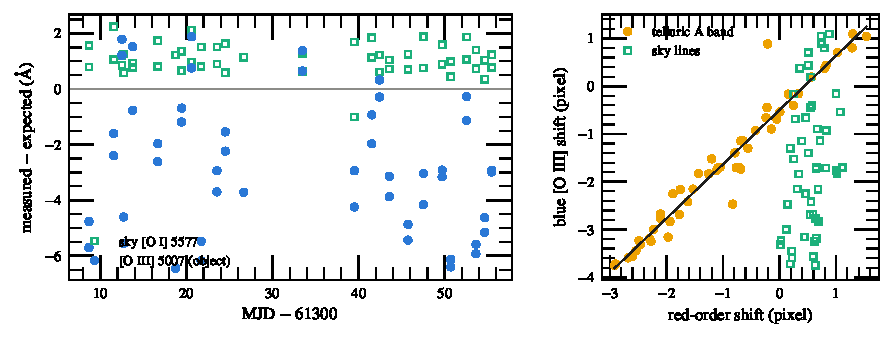
\includegraphics[width=\textwidth]{figures/fig_zeropoint.pdf}
\caption{Left: blue-order [O\,{\sc iii}] shift of Fairall~9 (filled) and 5577\,\AA{} sky-line shift (open) per exposure
in the archive products. Right: blue-order [O\,{\sc iii}] pixel shift against the red-order A-band (filled) and sky-line
(open) pixel shifts; the line has slope 1.13.}
\label{fig:zeropoint}
\end{figure}


After the arc refit and the telluric zero point (Fig.~\ref{fig:redshift}, Table~\ref{tab:summary}) the nuclear
narrow lines agree from exposure to exposure to 20--40\,\kms{} in both orders, and the two orders agree with each
other to $\approx10$\,\kms. Applying each night's own arc fit instead of the median correction increases the scatter
of the red--blue difference from 0.6 to 1.0\,\AA. This confirms that the shape of the arc solution is stable and that
the per-night fit only adds noise.

Two further tests support the method. (i) Before correction, the shifts of [O\,{\sc iii}] and [Ne\,{\sc iii}] follow
the applied zero point with slopes 0.94 and 0.96, whereas the Ca\,{\sc ii}\,K absorption of the host galaxy follows
it with slope 0.17. The host is extended and fills the slit, like the sky. The correction is therefore right for the
nuclear light that RM measures, but not for the host starlight, which matters for decompositions of the host
spectrum. (ii) In the corrected spectra, the cleaner red order yields [O\,{\sc i}]\,6300 in \OIN{} of the 50 spectra, at
\OIvel\,\kms, while [O\,{\sc iii}] sits at \OIIIvel\,\kms. [O\,{\sc iii}] is thus $\approx150$\,\kms{} bluer than
[O\,{\sc i}], a typical signature of an [O\,{\sc iii}] outflow; this bounds the absolute zero-point error at
$\approx2$\,\AA.

\begin{figure}[!htbp]
\centering
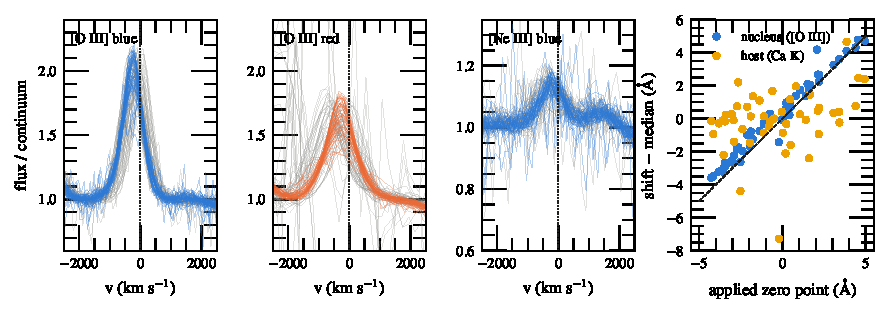
\includegraphics[width=\textwidth]{figures/fig_redshift.pdf}
\caption{Narrow lines of the 50 Fairall~9 spectra in velocity relative to $z=0.047016$: archive (grey) and this work
(colour). Right: shift in the archive products against the applied blue-order zero point for [O\,{\sc iii}] (nucleus)
and Ca\,{\sc ii}\,K (host); dashed: slope 1.}
\label{fig:redshift}
\end{figure}


